%!TEX root = ../main.tex
% Chapter 7

\chapter{Inhaltliche Konzeption des Systems}
\label{Inhaltliche_Konzeption_des_Systems}

Dieses Kapitel beschäftigt sich mit der inhaltlichen Konzeption des Systems, welches folgend auch Pay2Mail genannt wird. Der Fokus liegt auf der Interaktion des Nutzers mit dem System, organisatorischen Fragen, sowie einer Vorauswahl von Bezahl- und Tokensystemen, die in Kapitel xx zur Auswahl stehen.

\section{Auswahl von Bezahl- und Tokensystemen}
\label{Auswahl_von_Bezahl-_und_Tokensystemen}
In Kapitel \ref{Bezahlsysteme_zur_Schaffung_von_Vorteilen_in_Videospielen_(Pay_to_Win)} wurden verschiedene Zahlungsmodelle vorgestellt, mit denen in Videospielen ein Gegenwert erzeugt wird. Zu Beginn ist das Abonnement zu nennen, mit welchem ein Vorteil für einen Zeitraum unter der Voraussetzung der regelmäßigen Zahlungen erworben wird. Für Pay2Mail eignet sich dieser Ansatz nicht, da ein Abonnementspreis statisch wäre und sich nicht anhand des E-Mail Aufkommens verändert. Das bedeutet, dass eine E-Mail je nach Monat und Bearbeitungsleistung unterschiedliche Bearbeitungszeiten hätte, ohne dass Nutzer aktiv priorisieren könnten. Stattdessen kann nur eine generelle Tendenz zur Priorisierung gegeben werden, vergleichbar mit dem Express-Versand, den Logistikunternehmen anbieten. Ein weiterer Nachteil ist die fehlende Flexibilität. So eignet sich ein Abonnement nur für Nutzer, die einen kleinen Empfängerkreis haben, den sie häufig kontaktieren. Andernfalls müssten viele Abonnements abgeschlossen werden, was ineffizient und kostenaufwändig ist.

Statt eine laufendes Abonnement vorauszusetzen, könnten Zahlungen spezifisch pro E-Mail gesetzt werden. Der Vorteil ist, dass die Höhe abhängig vom Empfänger und dessen Aufkommen festgelegt werden kann. Außerdem ist, im Vergleich zu Abonnements ein individueller Betrag setzbar, ohne dass eine Preisstaffelung erfolgt. Auch ist dieses Vorgehen in der automatischen Triage effektiver, da Zahlungen miteinander verglichen werden können, ohne dass gleich hohe Abonnementspreise den Empfänger zwingen eine eigene Triage durchzuführen. 

Ein Nachteil von Zahlungen mit Echtgeld ist, dass eine Benachteiligung von Personen entsteht, die sich solche Zahlungen nicht leisten können, obwohl E-Mails versenden müssen, die eine hohe Priorität haben. Das führt dazu, dass nicht relevante E-Mails priorisiert werden, sondern E-Mails von Personen, die sich eine Priorisierung leisten können. Dies ist insbesondere bei Empfängern mit einem sehr hohen Aufkommen und/oder geringer Bearbeitungsleistung der Fall. Um diese soziale Diskrepanz zu begleichen bieten sich token-basierte Gegenwerte an. Absender erhalten für einen fest definierten Zeitraum eine Anzahl an Token, welche sie als Gegenwert setzen können. Somit ist der finanzielle Stand eines Absenders irrelevant, vielmehr zählt wie er seine Token verwendet. Das Tokensystem ist dem Konzept des \acrshort{lcp} aus Kapitel \ref{Payment-Based_Email} nachempfunden. 

Ein Tokensystem löst zwar die soziale Ungleichheit in der Priorisierung von Absendern aus, sorgt allerdings auch dafür, dass Token nicht so verteilt sind, wie sie benötigt werden. Es gibt Absender, die eine größere Anzahl an E-Mails, auch priorisiert, versenden wollen als es der durchschnittliche Absender würde. Solche Intensivnutzer hätten mit dem Tokensystem keine Möglichkeit ihr hohes Sendeaufkommen vollständig zu priorisieren. Absender mit wenigen E-Mails hingegen können eine unproportional große Anzahl an Token auf wenige E-Mails setzen und sich durch ihre geringe Nutzung einen Vorteil verschaffen. Eine Kombination aus Echtgeldzahlungen und Token würde dieses Problem lösen. Das bedeutet, dass jeder Nutzer eine spezifische Anzahl an ''Grundtoken'' erhält, um E-Mails unabhängig von der eigenen finanziellen Situation priorisieren zu können. Nutzer mit viele E-Mails können darüber hinaus weitere Token erwerben, um ihrem hohen Bedarf gerecht zu werden. Wichtig ist hierbei, dass die Token einen festen und unveränderlichen Preis haben. Dadurch können intransparente Preisstrukturen und kasino-ähnliche Verhaltensweisen, wie in Kapitel \ref{Bezahlsysteme_zur_Schaffung_von_Vorteilen_in_Videospielen_(Pay_to_Win)} erläutert, vermieden werden, was die Vertrauenswürdigkeit von Pay2Mail erhöht.

Somit werden den Befragten in Kapitel xx drei Bezahl- und Tokensysteme vorgeschlagen: Priorisierung von E-Mails mit Echtgeld; Setzen von Token, die jeder Nutzer in gleicher Menge erhält oder die Erweiterung dessen mit der Option Token mit Echtgeld nachzukaufen.

%----------------------------------------------------------------------------------------

\section{Use Cases}
\label{Use_Cases}
Im Folgenden werden Anwendungsfälle (Use Cases) definiert, die dazu dienen die Bedürfnisse des Nutzers, seine Interaktion, sowie seinen gewünschten Zielzustand festzuhalten.

\subsection*{Use Case 1: Priorisierung einer E-Mail}
\textbf{Akteur}: Absender einer E-Mail \\
\textbf{Vorbedingung}: Der Empfänger hat Pay2Mail konfiguriert und nutzt es aktiv. \\
\textbf{Auslöser}: Nutzer muss eine E-Mail versenden, die priorisiert bearbeitet werden soll. \\
\textbf{Endzustand im Erfolgsfall}: Nutzer hat die E-Mail mit einem Gegenwert versendet. \\
\textbf{Endzustand im Fehlerfall:} Nutzer konnte keinen Gegenwert an die E-Mail anhängen und hat sie unpriorisiert versendet. \\

\noindent \textbf{Normaler Ablauf}:
\begin{enumerate}
    \item Nutzer öffnet einen Mailclient seiner Wahl.
    \item Nutzer trägt den Empfänger der E-Mail ein.
    \item Nutzer erhält die Information zur möglichen Priorisierung.
    \item Nutzer öffnet die Oberfläche zur Priorisierung und zahlt Geld/Token.
    \item Nutzer erhält E-Mail Header zur Bestätigung der Zahlung.
    \item Nutzer setzt E-Mail Header und füllt die restlichen Felder aus.
    \item Nutzer versendet die E-Mail.
\end{enumerate}

\noindent \textbf{Erweiterungen}:
\begin{enumerate}
\setcounter{enumi}{3}
    \item a) Nutzer sieht sich vor der Zahlung das E-Mail Aufkommen an, um eine Entscheidung über die Höhe des Gegenwerts zu treffen.
\end{enumerate}

\noindent \textbf{Variationen}:
\begin{enumerate}
\setcounter{enumi}{5}
    \item \textquotesingle{} Nutzer setzt den Header nicht selbst, stattdessen wird er automatisch ausgefüllt.
\end{enumerate}


\subsection*{Use Case 2: Einsicht in das E-Mail Aufkommen eines Empfängers}
\textbf{Akteur}: Absender einer E-Mail \\
\textbf{Vorbedingung}: Der Empfänger hat Pay2Mail konfiguriert und nutzt es aktiv. \\
\textbf{Auslöser}: Nutzer ist interessiert daran, wie lange er auf eine Antwort warten muss. \\
\textbf{Endzustand im Erfolgsfall}: Nutzer kennt das E-Mail Aufkommen des Empfängers und kennt die potenzielle Bearbeitungszeit. \\
\textbf{Endzustand im Fehlerfall:} Nutzer kann die potentielle Bearbeitungszeit nicht ermitteln. \\

\noindent \textbf{Normaler Ablauf}:
\begin{enumerate}
    \item Nutzer öffnet einen Mailclient seiner Wahl.
    \item Nutzer trägt den Empfänger der E-Mail ein.
    \item Nutzer erhält die Information zur möglichen Priorisierung.
    \item Nutzer öffnet die Oberfläche zur Priorisierung.
    \item Nutzer wählt die Auflistung des Aufkommens mit Bearbeitungszeit aus.
    \item Nutzer kann die Bearbeitungszeit je nach Gegenwert ablesen.
    \item Nutzer schließt die Oberfläche und den Mailclient.
\end{enumerate}

\noindent \textbf{Erweiterungen}:
\begin{enumerate}
\setcounter{enumi}{5}
    \item a) Nutzer zahlt Geld oder setzt einen Token, siehe ab Schritt 5 von Use Case 1.
\end{enumerate}

\noindent \textbf{Variationen}:
\begin{enumerate}
\setcounter{enumi}{4}
    \item \textquotesingle{} Nutzer sieht nicht die Bearbeitungszeit, sondern die Bearbeitungsleistung des Empfängers.
\end{enumerate}


\subsection*{Use Case 3: Automatische Triage des Posteingangs}
\textbf{Akteur}: Empfänger von E-Mails \\
\textbf{Vorbedingung}: Der Empfänger hat Pay2Mail konfiguriert. \\
\textbf{Auslöser}: Nutzer will/muss seine E-Mails bearbeiten und sein Postfach kontrollieren. \\
\textbf{Endzustand im Erfolgsfall}: Der Posteingang ist sortiert und der Nutzer weiß unmittelbar welche E-Mails er wann bearbeiten muss. \\
\textbf{Endzustand im Fehlerfall}: Der Posteingang ist unsortiert und der Nutzer muss die Triage selbst durchführen. 

\newpage

\noindent \textbf{Normaler Ablauf}:
\begin{enumerate}
    \item Nutzer öffnet die Anwendung.
    \item Nutzer sieht die zu bearbeitenden E-Mails in sortierter Form.
    \item Nutzer bearbeitet E-Mails entsprechend seiner Bearbeitungsleistung.
    \item Nutzer schließt die Anwendung.
\end{enumerate}

\noindent \textbf{Erweiterungen}:
\begin{enumerate}
\setcounter{enumi}{2}
    \item a) Nutzer entscheidet sich weniger priorisierte E-Mails zu bearbeiten, die nicht zur Bearbeitungsleistung gezählt werden, aber für ihn relevant sind.
\end{enumerate}

\noindent \textbf{Variationen}: \\
-

%----------------------------------------------------------------------------------------

\section{Content Model}
\label{Content_Model}
Das Content Model beschreibt die Struktur der Inhalte in einer Anwendung. Dabei unterscheidet es sich von Datenmodellen, wie einem UML-Klassendiagramm, dadurch, dass die Formulierung bewusst un-technisch ist und keinerlei Einfluss auf die Technologieentscheidung und Implementation hat. Durch die Domäne \textit{E-Mail} sind gewisse technische Begriffe notwendig, diese werden jedoch minimal gehalten und bleiben unspezifisch hinsichtlich der Implementation. 

\begin{figure}[!ht]
	\centering
		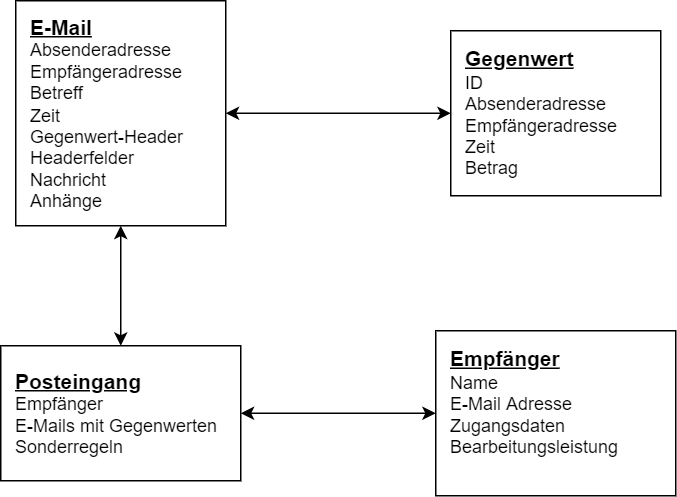
\includegraphics[width=0.75\textwidth]{Figures/Content Model.png}
	\caption{Content Model}
	\label{fig:content_model}
\end{figure}

\noindent Abbildung \ref{fig:content_model} zeigt das Modell. Als übergeordnetes Element kann der Posteingang verstanden werden, der pro Empfänger einmalig ist. Er enthält Informationen zum Empfänger, den E-Mails mit ihren Gegenwerten und Sonderregeln. Sonderregeln sind die in Kapitel \ref{Anforderungen_von_Empfaengern} thematisierten Abweichungen von der automatischen Triage. Der Empfänger besteht aus persönlichen Daten, sowie der Bearbeitungsleistung, die für die Einsicht relevant ist. Der Absender wurde im Content Model vernachlässigt, da er lediglich als E-Mail Adresse Teil des Systems ist; weitere Informationen über ihn sind nicht erforderlich. Die E-Mail enthält die für sie typischen Felder und den Gegenwert-Header, wie er in Kapitel \ref{Erkenntnisse_fuer_das_zu_entwickelnde_System} konzipiert wurde. Der Header enthält einen eindeutigen Identifikator, um den Gegenwert zuzuordnen. Dieser enthält grundlegende Informationen zur E-Mail, sowie den hinterlegten Betrag als Währung und Token.


%----------------------------------------------------------------------------------------

\section{Navigation Model}
\label{Navigation_Model}

Das Navigation Model beschreibt die einzelnen Bestandteile der Nutzeroberfläche und ihre Navigierbarkeit anhand von Pfeilen. Dabei unterscheidet es sich von Sequenzmodellen, wie einem UML-Ablaufdiagramm, dadurch, dass die Formulierung bewusst un-technisch ist und keinerlei Einfluss auf die Technologieentscheidung und Implementation hat. Da sich die Oberflächen für Absender und Empfänger grundlegend unterscheiden, werden zwei Modelle verwendet.

\begin{figure}[!ht]
	\centering
		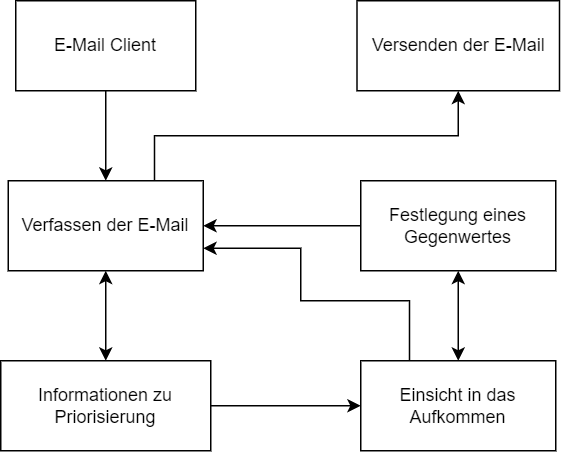
\includegraphics[width=0.75\textwidth]{Figures/Navigation Model Absender.png}
	\caption{Navigation Model des Absenders}
	\label{fig:navigation_model_absender}
\end{figure}

\noindent Das Navigation Model des Absenders in \ref{fig:navigation_model_absender} orientiert sich an den Use Cases 1 und 2. Es ist abhängig vom Mailclient, daher sind Abweichungen möglich. Grundlegend wird der Client gestartet und die Oberfläche zum Verfassen einer E-Mail aufgerufen. Der Nutzer erhält nach Eingabe des Empfängers die Information, dass Pay2Mail verwendet wird. Er kann diesen Hinweis ausblenden oder sich das Aufkommen des Empfängers ansehen. Hier hat er die Möglichkeit zurückzukehren oder einen Gegenwert zu hinterlegen, wobei er zurück zum Verfassen der E-Mail geleitet wird. Hier kann er, abhängig vom Client, die E-Mail vervollständigen und abschließend versenden.

\begin{figure}[!ht]
	\centering
		\includegraphics[width=0.75\textwidth]{Figures/Navigation Model Empfänger.png}
	\caption{Navigation Model des Empfängers}
	\label{fig:navigation_model_empfaenger}
\end{figure}

Das Navigation Model des Empfängers (siehe Abbildung \ref{fig:navigation_model_empfaenger} ist nicht prozessorientiert, daher ist die Navigation stets bidirektional. Zu Beginn erscheint die Liste der E-Mails, wobei die Triage bereits durchgeführt wurde. Der Nutzer kann eine E-Mail in der Liste auswählen und die Bearbeitung, bzw. Beantwortung beginnen. Hier können Abweichungen an der Priorität gesetzt werden, die vom Posteingang gespeichert werden. Außerhalb der Bearbeitung von E-Mails kann der Nutzer Sonderregeln definieren, die automatisch Abweichungen von der Triage vornehmen. Darüber hinaus können Einstellungen an der Anwendung vorgenommen werden, wie die eigene Bearbeitungsleistung zu verändern. Jeder Schritt ermöglicht es zurück zur Liste der E-Mails zurückzukehren.

Dadurch, dass die technische Konzeption an diesem Punkt noch aussteht, ist die inhaltliche Konzeption als Grundlage, jedoch nicht als festes Regelwerk zu verstehen. Es ist möglich, dass sich die Navigation im System während der Implementation verändert. Abweichungen von der inhaltlichen Konzeption werden an entsprechender Stelle festgehalten und begründet.